\section{Modeling, Analyzing and Slicing Periodic Distributed Computations \\ 
\small{Vijay K. Garag, Anurag Agarwal, Vinit Ogale}}

\subsection{Notes}

This paper proposes an anaylsis technique for decomposing distributed
exectutions. It proposes a very interesting model, in which DAG's are infinine.
Their proposed infanite DAG is reffered to as a \textit{d-diagram} and
essentially models looping computation post predicate on an infanite timeline.
They use this model to verify temporal properties such as liveness.

Not the useage of \textit{cut frontier}. This is proper usage and should be
intagrated into the \dinv paper if possible.

A very interesting addition on page 14 is the formalization of recursive vector
closk. It is simple algebra, but it states simply that given some initial
configuration $C$ lets say, and a continuing recursive computation, the vector
clock values for all events, of future computations can be computed a priori.

The paper continues by formulating how to verify liveness properties 

\subsection{Observations}

My immidate impression of this paper is that it falls short in its model of a
distributed execution. It only defines an infanite execution as a prefix
followed by a periodic set of recurrent transitions. It seems that this model
is strictly limited to a single periodic computation, and not a general
computation which must adapt to interaction.

For instance this model could be used to analyze a key value store which only
serverd puts, or gets, or a fininte repeatable sequence of accesses. It would
however fall short in the following scenarios.

I was interested in extending the model presented in this paper. As mentioned
in the prior paragraph there are a few shortcommings, such as the models
ability to only quantify a single infanite state. I drafted an extension to
this model on the board. 

\begin{figure}[t]
    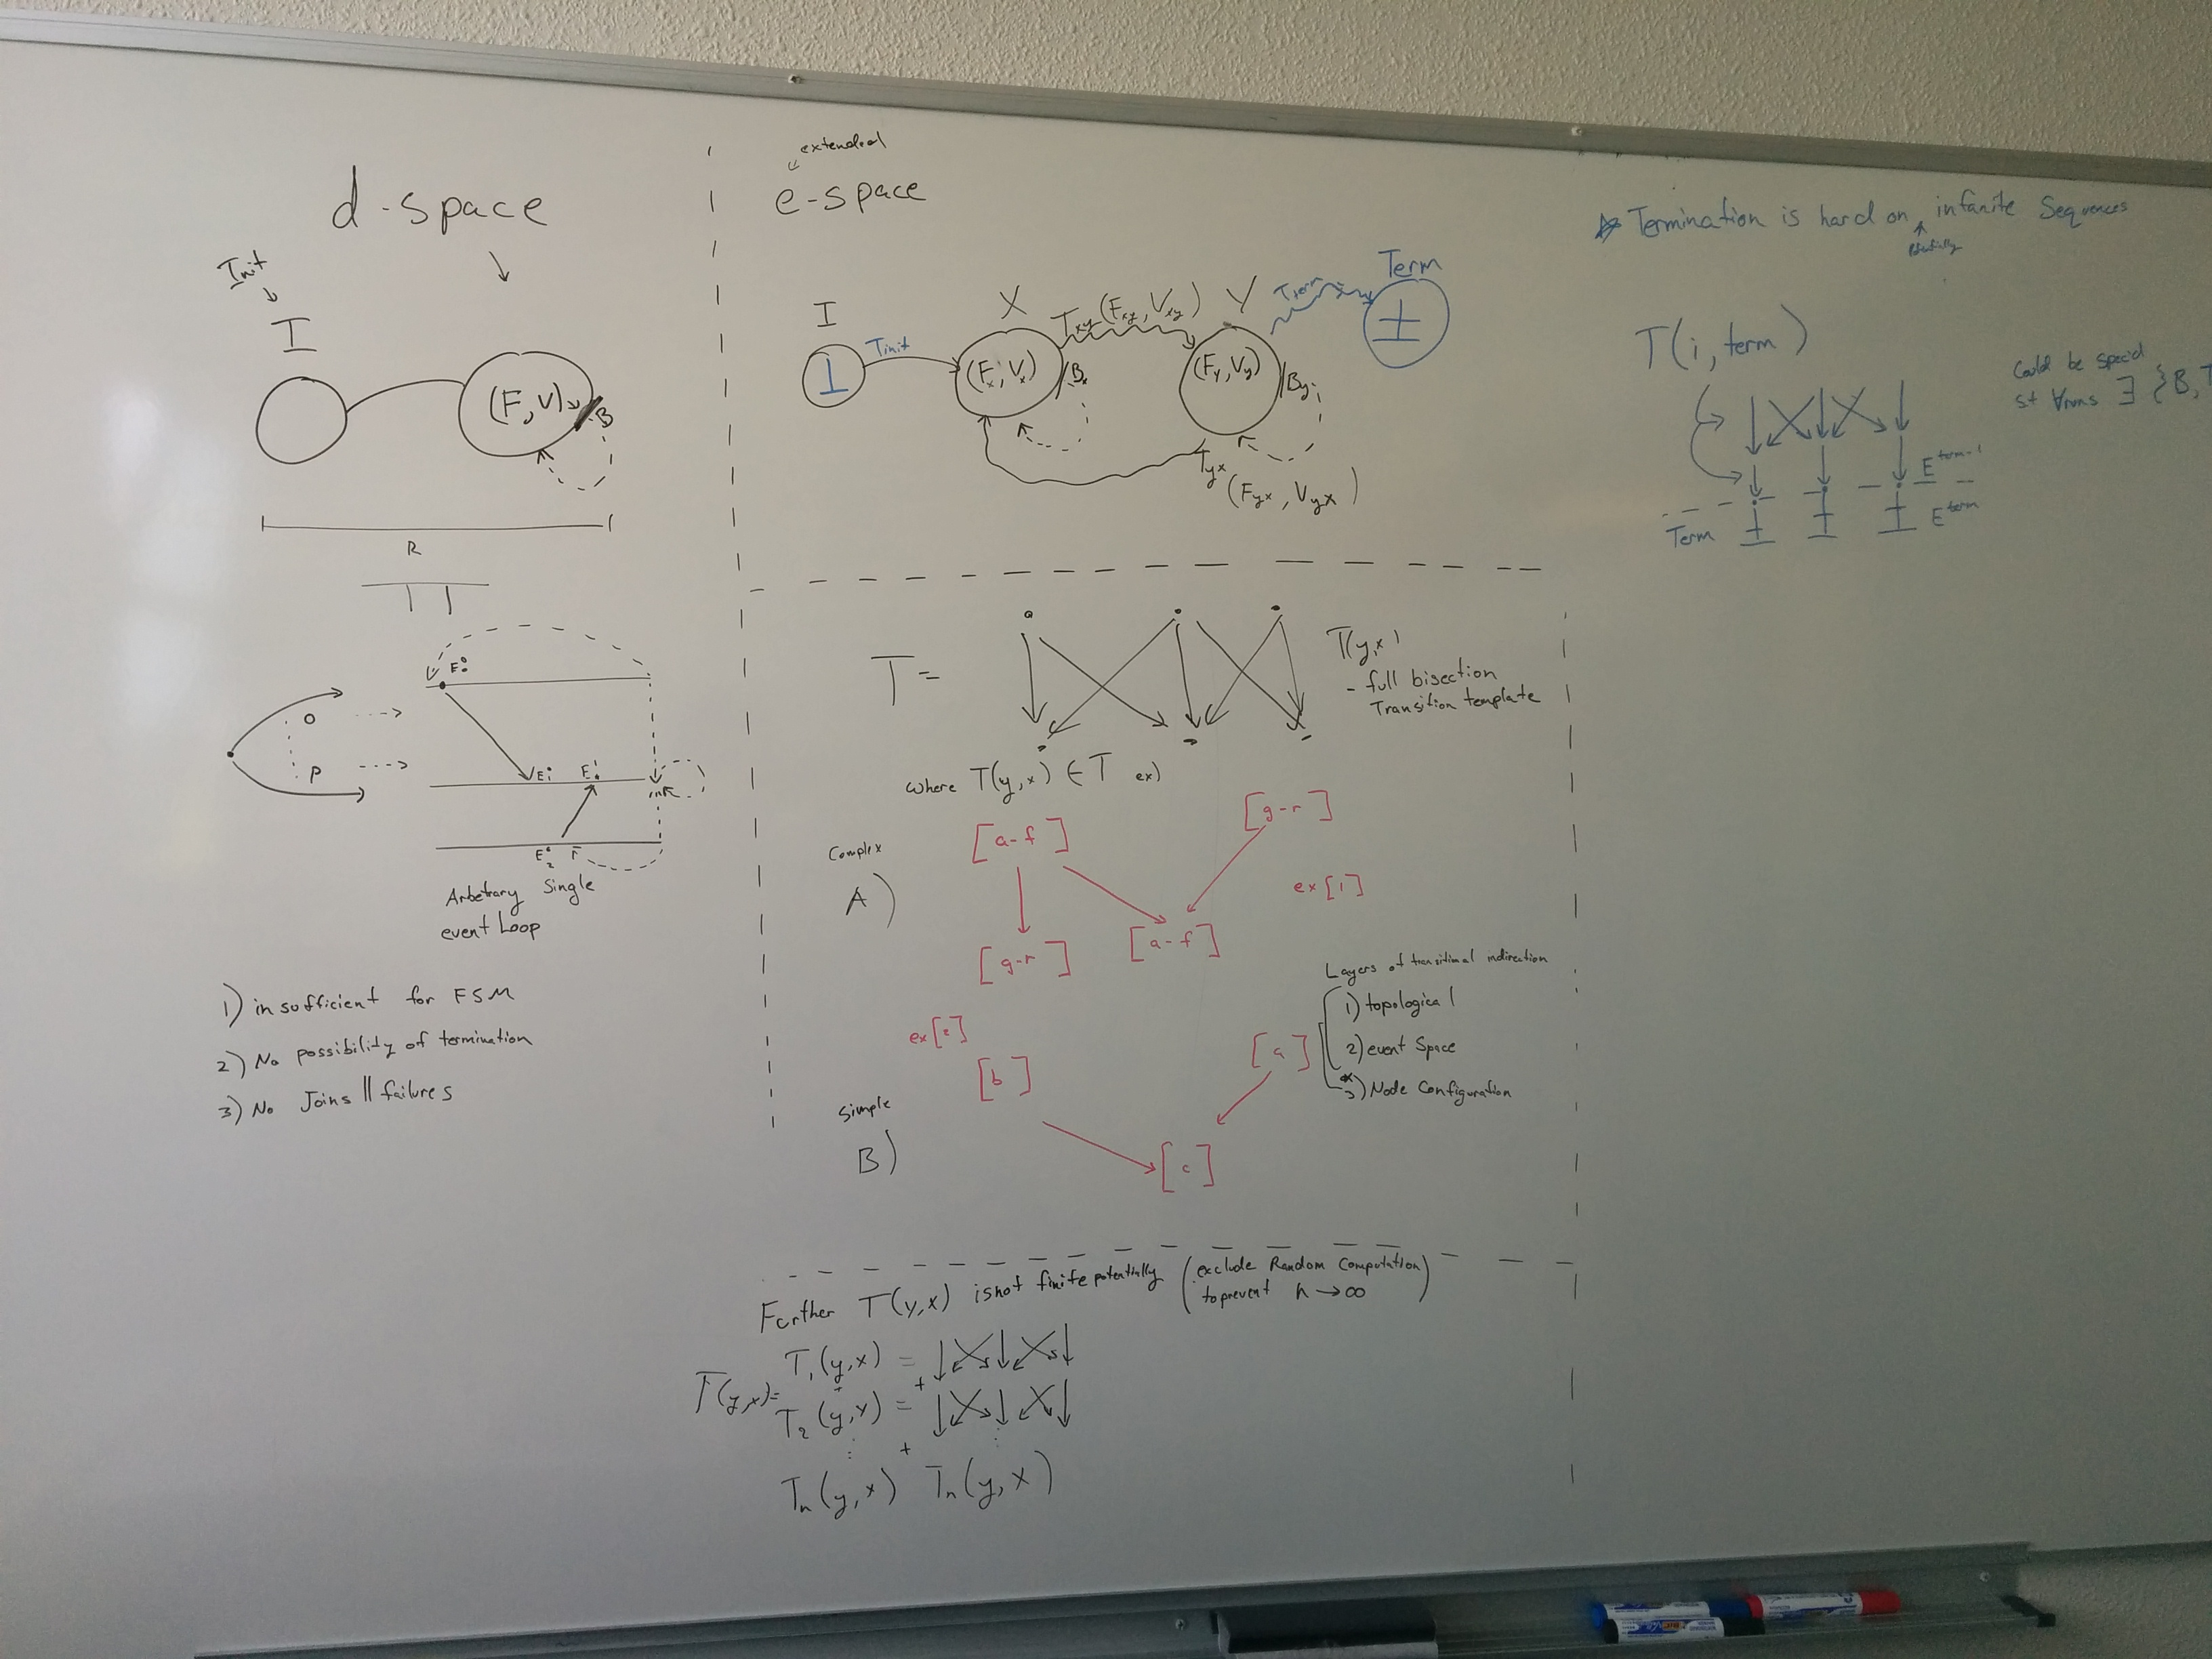
\includegraphics[width=0.50\textwidth]{fig/espace}

    \caption{Sketch of a potential extension to the d-diagram model}

\label{fig:espace} 
\end{figure}


\begin{itemize}

\item{addition of new nodes}

\item{failure of a node}

\item{loss of messages \textit{I think?}}

\item{non deterministic accesses}

\item{Recovery / Fault detection / Reconfiguration}

\end{itemize}

I believe that a more complete model would generalize \textit{d-diagrams} to be
similar to lego blocks, or components of a generalized state machine of a
computation (but I'll finish the paper before jumping on this).


